\chapter{Introduction}
\label{ch:intro}

This chapter sets out the motivation, problem statement, objectives, and scope of the work presented in this thesis, and closes with a short map of how the remaining chapters are organised.

\section{Background and Motivation}

Drone-based radar search-and-rescue operates on a deceptively simple premise: a drone carries a radar sensor over a disaster area, detects breathing signatures beneath rubble, and displays the locations on a rescue map for first responders. The difficulty lies not in the radar itself but in the spatial reasoning layer that makes those detections \emph{actionable}.

A radar detects a human breathing signature and reports it as a range bin --- ``something is at 13.7\,meters.'' But the drone is moving forward at 2--5\,m/s and shifting due to wind. Range bin 47 at time $T_1$ does not map to the same physical spot on the ground as range bin 47 at time $T_2$. Without instantly translating local radar detections into global GPS coordinates by factoring in the drone's exact attitude (roll, pitch, yaw) and velocity at the exact microsecond of the radar sweep, the rescue map drifts by meters. A rescue team digs in the wrong place.

This translation --- \emph{radar-inertial georeferencing} --- requires tight attitude-to-radar synchronization. The drone's flight controller produces attitude and position estimates at 100\,Hz via the MAVLink protocol. The radar produces range-Doppler target lists at 10--50\,Hz. These two data streams must be fused in real time, with sub-millisecond temporal alignment, to produce drift-compensated target positions.

A Linux companion computer (Jetson, Raspberry Pi) cannot reliably perform this fusion. Operating-system scheduling jitter introduces milliseconds of latency spikes --- an eternity when the drone moves centimetres in that time. The georeferencing computation needs a \emph{deterministic} execution environment with guaranteed response times. This is where a bare-metal microcontroller becomes indispensable.

The target device is the STM32H753, built around an Arm Cortex-M7 core clocked at up to 480\,MHz. It provides deterministic, low-latency peripheral handling: DMA for zero-copy UART ingestion, hardware timers with input capture for microsecond-precise timestamping, a hardware CRC peripheral for packet integrity verification, and a Memory Protection Unit for memory safety --- all executing without an operating system. The Cortex-M7's L1 caches, double-precision FPU, and CMSIS-DSP matrix libraries make it capable of running a 6-state Extended Kalman Filter at the required rate.

The specific defects reproduced in this thesis are not algorithmic errors in the EKF or coordinate transform mathematics. They are the systems-level failures that emerge when firmware, compiler, and hardware interact: a DMA transfer that bypasses the L1 data cache leaving the CPU reading stale data, a compiler struct-padding mismatch that silently shifts all floating-point fields, a hardware timer prescaler that doesn't load without an explicit update event, an EKF matrix multiplication that aliases its own input buffers, and a coordinate transform that rotates in the wrong direction because a quaternion conjugate was applied incorrectly. Each defect looks correct at the level of the C source; each is wrong only once the silicon's bus behaviour, the compiler's layout rules, or the FPU's memory access patterns are taken into account.

\section{Problem Statement}

A bare-metal firmware stack for deterministic radar-inertial georeferencing on an Arm Cortex-M7 microcontroller must ingest high-rate MAVLink telemetry, hardware-timestamp radar frames, fuse them through an Extended Kalman Filter, georeference the targets, and stream results --- all within hard real-time constraints and without an operating system. Each pipeline stage --- DMA-based MAVLink parsing, timer-synchronized timestamping, lock-free inter-stage buffering, EKF prediction and update, quaternion-based coordinate transformation, and deterministic output framing --- introduces specific failure modes that are invisible to code review and manifest only in silicon.

A systematic, case-by-case verification methodology is required to find and resolve these failures before they reach a field deployment. The methodology must use deterministic, open-source emulation as its primary tool, remain explicitly aware of where that emulation diverges from physical silicon, and confirm its findings with hardware-in-the-loop testing using real data.

\section{Objectives}

\begin{enumerate}
\item Design and implement a deterministic radar-inertial georeferencing coprocessor firmware stack on the STM32H753, covering zero-copy DMA-based MAVLink ingestion, hardware-timer radar frame timestamping, lock-free kinematic state buffering, 6-state EKF sensor fusion, quaternion-based coordinate transformation (polar$\rightarrow$ENU$\rightarrow$WGS84), and deterministic binary output streaming.
\item Establish Renode, an open-source deterministic hardware emulator, as the primary reproducible verification environment for every pipeline stage.
\item Generate hardware-in-the-loop test stimuli using real MAVLink v2 packets (via pymavlink) with correct protocol CRCs, inject them into the simulation, and verify end-to-end georeferenced output.
\item Identify, reproduce, and root-cause eleven classes of genuine embedded-systems defects spanning build-system path resolution, interrupt controller register naming, bare-metal C library linking, DMA-to-CPU cache coherency, struct-packing alignment, timer prescaler shadow loading, interrupt priority ordering, memory barrier requirements, EKF matrix buffer aliasing, quaternion rotation direction, output frame length calculation, and MAVLink parser packet boundary management.
\item Explicitly identify and document concrete divergences between the Renode functional model and physical STM32H753 silicon, and engineer the firmware defensively wherever such a divergence is found.
\end{enumerate}

\section{Scope and Limitations}

The scope of this thesis is precisely the five objectives above, verified primarily through Renode simulation with hardware-in-the-loop testing using real MAVLink data. Several adjacent goals are explicitly \textbf{out of scope}:

\begin{itemize}
\item This work targets a specific drone-based radar search-and-rescue scenario. The georeferencing pipeline is designed for this use case and may require adaptation for other radar platforms or drone configurations.
\item The firmware parses three MAVLink message types (ATTITUDE, LOCAL\_POSITION\_NED, GLOBAL\_POSITION\_INT) relevant to georeferencing, not the full MAVLink message set.
\item No formal worst-case execution time (WCET) analysis is performed; timing is verified through simulation and architectural reasoning.
\item Physical-hardware testing is limited to the constraints of the Renode simulation model. The firmware is engineered defensively for silicon correctness where the emulator diverges (cache coherency, timer input capture, CRC hardware), but full physical-hardware validation is not performed.
\item The EKF uses a simplified 6-state model (position + velocity) with attitude fused separately via quaternion. A full 9-state or 15-state EKF including bias estimation is not implemented.
\end{itemize}

\section{Thesis Organisation}

The remainder of this thesis is organised as follows. Chapter~2 reviews the background material a reader needs: radar georeferencing principles, MAVLink telemetry protocol, DMA-based data ingestion, the Cortex-M7 cache architecture, Extended Kalman Filter theory, quaternion-based coordinate transforms, and hardware-in-the-loop verification methodology. Chapter~3 presents the system architecture: requirements, target platform, memory map, pipeline stages, data flow, and verification toolchain. Chapter~4 is the empirical core: eleven pipeline-stage case studies, each isolating a specific capability, the defect it exposed, and the verified resolution. Chapter~5 presents the Renode verification results including hardware-in-the-loop testing with real MAVLink data, documents the simulator-versus-silicon fidelity gaps, and discusses limitations. Chapter~6 concludes and outlines future work.

Figure~\ref{fig:1.1} previews the pipeline progression. Each stage adds one capability and, in doing so, exposes exactly one new way for the system to fail --- the defect that the corresponding case study in Chapter~4 reproduces and resolves.

\begin{figure}[htbp]
\centering
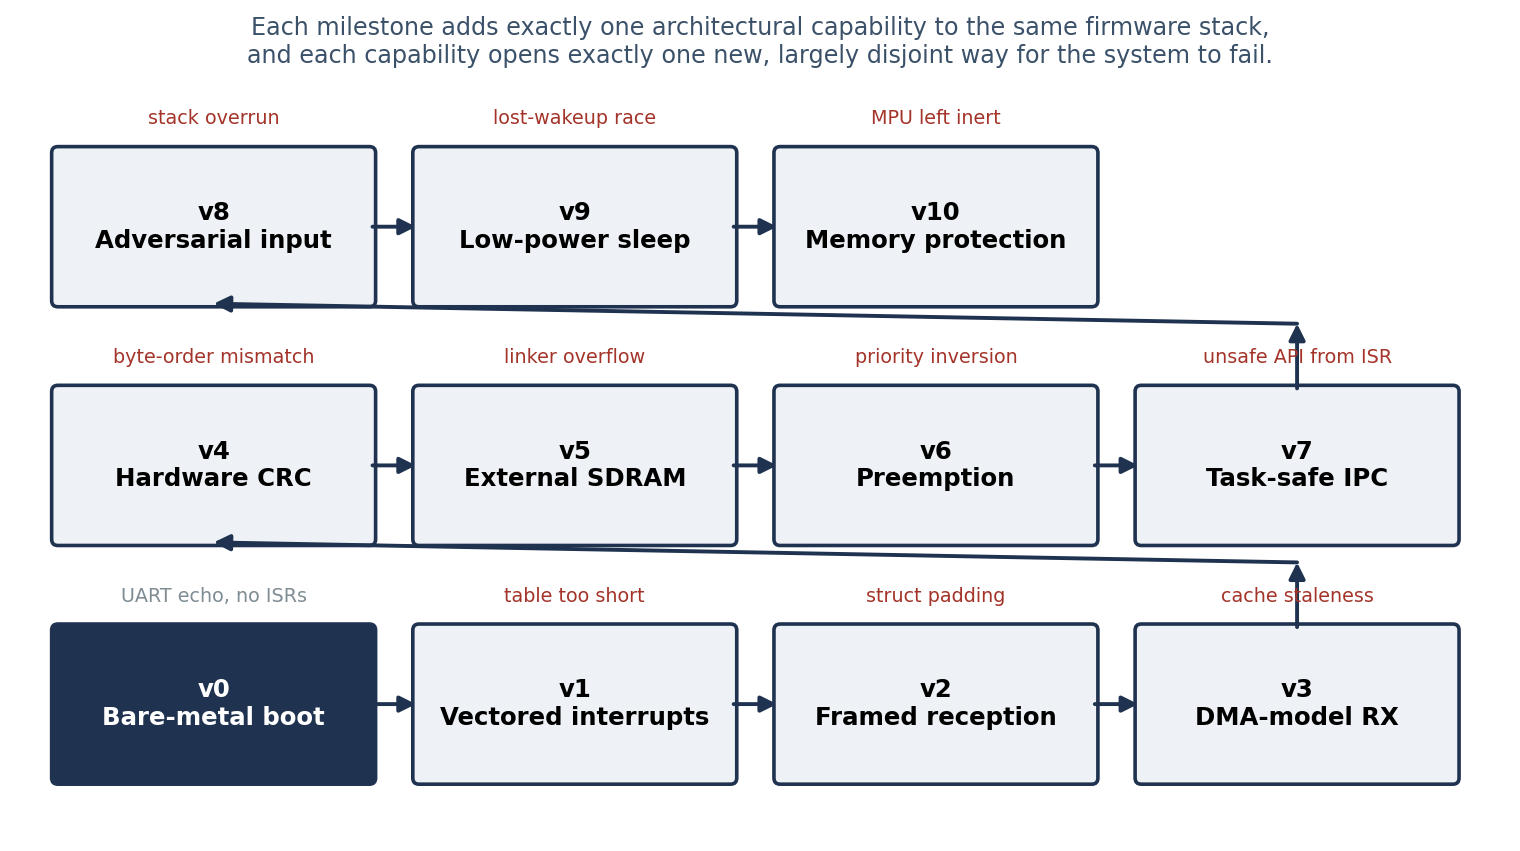
\includegraphics[width=0.98\textwidth]{figures/fig_1_1_milestone_roadmap.png}
\caption{The eleven-case study progression this thesis follows. Each stage adds one pipeline capability and exposes exactly one new failure mode (Chapter 4).}
\label{fig:1.1}
\end{figure}